\section{Dataset Description}

The field campaign was conducted in a freshwater environment in the Amazon region (Itacoatiara, AM, Brazil), with georeferenced sampling points distributed to capture local spatial gradients. The dataset includes position in UTM 21S and physicochemical variables used as model inputs and outputs. The spatial coverage of the campaign is shown in Fig.~\ref{fig:dataset_map}, and summary statistics of the prediction targets are reported in Table~\ref{tab:dataset_stats}.

Data collection followed a spatially distributed design to represent different lake micro-zones instead of repeatedly sampling a single coordinate. This choice was aligned with the study goal of supporting spatial interpretation and local decision support, including interpolation maps and composite screening indices. Measurements were consolidated into a tabular structure suitable for edge-oriented inference workflows and reproducible model training.

\subsection{Variables and Acquisition}
Input features were $x$, $y$, temperature (TEMP), apparent color in amber scale (COR\_A), and visual color index (COR\_V). Target variables were pH, dissolved oxygen (OD), and turbidity (TURB). The sampling design prioritized spatial representativeness over dense temporal repetition, consistent with the objective of generating interpretable spatial surfaces.

\begin{figure}[t]
\centering
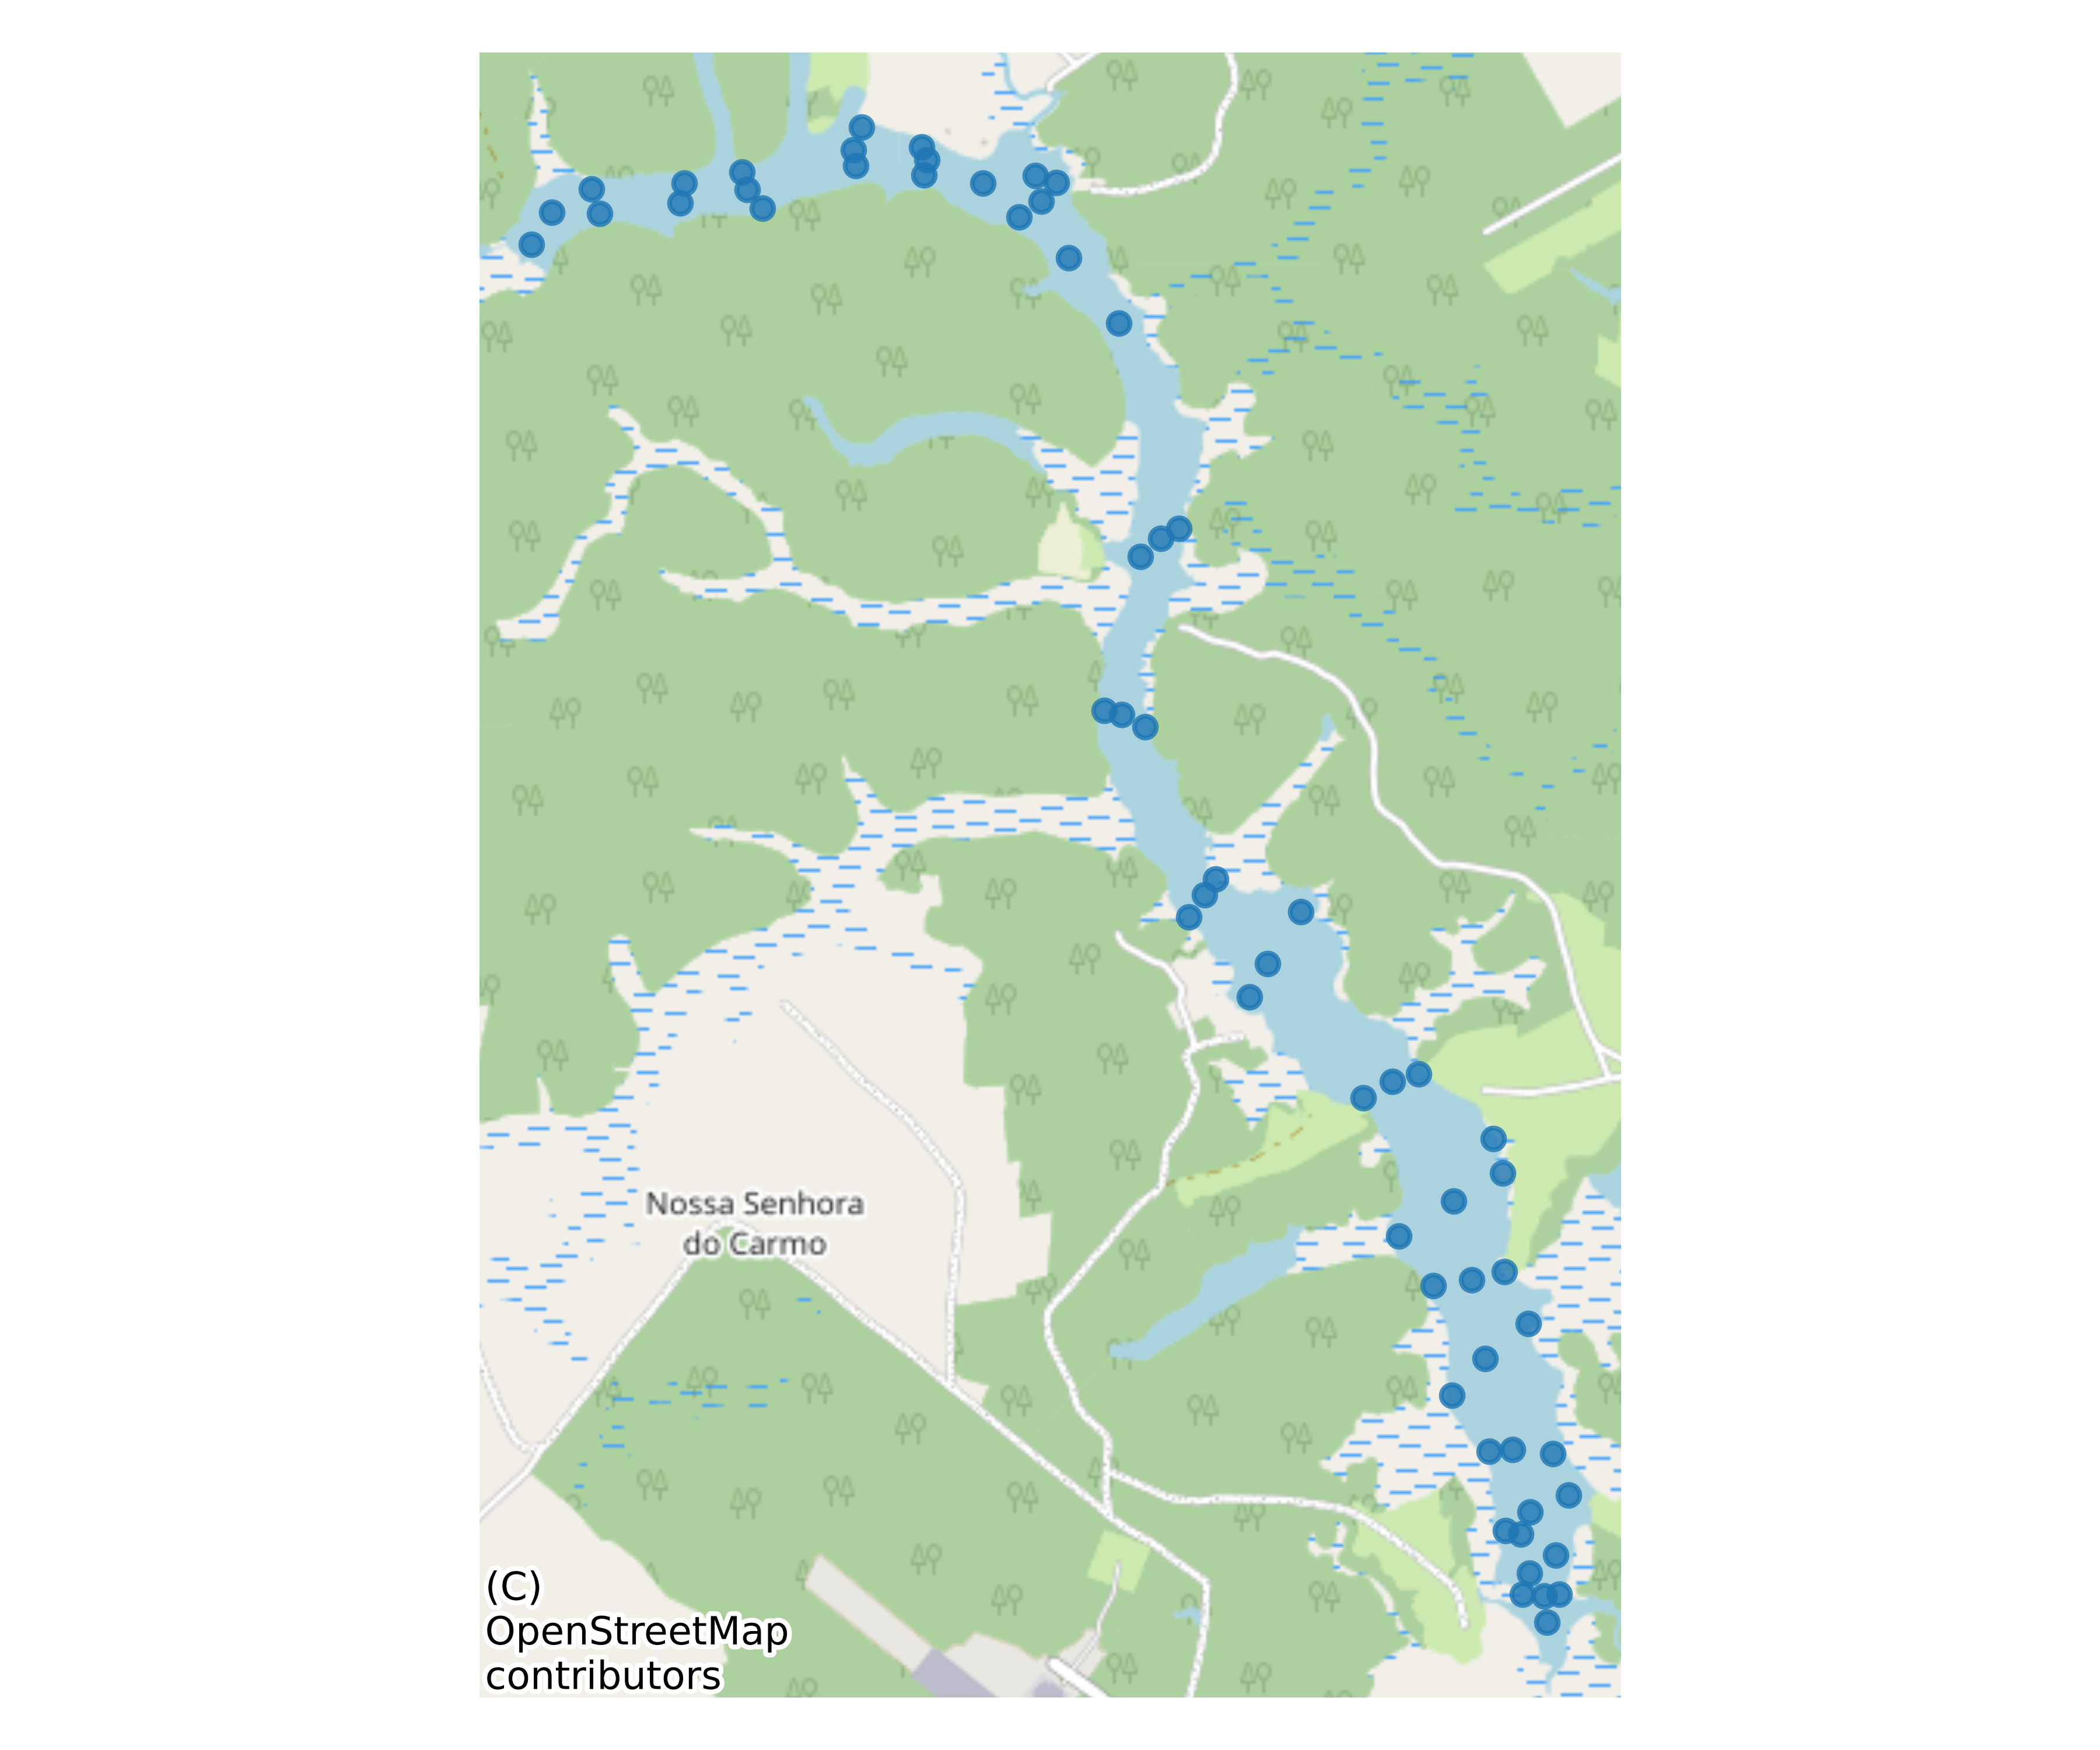
\includegraphics[width=0.78\textwidth]{map_points_osm_21S.png}
\caption{Sampling locations over OpenStreetMap basemap (UTM 21S).}
\label{fig:dataset_map}
\end{figure}

\begin{table}[t]
\caption{Target summary statistics in the original field dataset.}
\label{tab:dataset_stats}
\centering
\begin{tabular}{lcccc}
\toprule
Variable & Mean & Std & Min & Max \\
\midrule
pH & 5.73 & 0.31 & 5.15 & 6.50 \\
OD (mg/L) & 1.86 & 0.32 & 1.26 & 2.52 \\
Turbidity (NTU) & 2.77 & 1.37 & 0.06 & 6.18 \\
\bottomrule
\end{tabular}
\end{table}

\subsection{Data Augmentation}
Because the original dataset is small, synthetic augmentation was applied with factor $\times 10$ using light Gaussian perturbation ($\sigma=0.01$) in normalized space. This strategy was used to stabilize training and reduce split sensitivity, while preserving marginal distributions and physical plausibility. The augmented set is used for training support only and does not represent additional field measurements.

To minimize distortion risk, augmentation was constrained to low-amplitude perturbations and evaluated with distributional checks and ablation analysis. The objective was not to create synthetic dynamics absent from the field campaign, but to increase local density around observed samples and improve optimization stability across randomized splits. In practice, this reduced macro-MAE variability while preserving the same overall value ranges and central tendencies of the original measurements.

Finally, the dataset should be interpreted as an initial regional benchmark rather than a universal hydrological representation. The current sampling supports comparative modeling and deployment analysis, while broader external generalization requires multi-season campaigns and additional freshwater sites with different hydrodynamic and anthropogenic profiles.
